\chapter{State of the art}

Humans and other living beings, such as animals and plants, are complex multicellular organisms \cite{Knoll2011}. At the most fundamental level, cells serve as the building blocks of life \cite{O’ConnorAdams2010}. In animals, cells organize into tissues, organs, and organ systems. These systems work in concert to ensure the organism's survival, with their activities often regulated by the endocrine and nervous systems \cite{TortoraDerrickson2016}. Both the endocrine and nervous systems employ chemical messengers. The endocrine system utilizes hormones, which are released into the bloodstream to reach distant target sites. In contrast, the nervous system employs neurotransmitters, which are transmitted mainly through neuronal axons directly to target areas, exhibiting greater specificity and speed \cite{Kandeletal2000}.

Among these systems, the nervous system stands out as the most complex. It serves to coordinate motor and sensory information, transmitting signals between the brain and the rest of the body. Additionally, it plays a vital role in regulating various involuntary bodily functions, such as heartbeat, breathing, blushing, sweating, and blinking \cite{Dharani2015}.

In vertebrates (including humans) the nervous system is divided into two main parts: the central nervous systems (CNS), made up of the brain and spinal cord; and the peripheral nervous system (PNS), made up of nerves \cite{Kandeletal2000}. The nervous tissue is very delicate and even though the CNS is protected by bones and meninges, suspended in cerebrospinal fluid and isolated from the bloodstream by the blood–brain barrier, it is still susceptible to injuries, infections, and diseases.

Any type of brain damage that occurs after birth is called Acquired Brain Injury (ABI). ABIs don't include brain trauma at birth, congenital disorders or degenerative diseases - e.g. Alzheimer's disease, Parkinson's disease, Huntington's disease, Multiple sclerosis, Amyotrophic lateral sclerosis, etc. An ABI can be considered either a Traumatic Brain Injury (TBI) - caused by an external force, e.g. motor vehicle accidents, falls, sports-related injury, and violence - or a Non-Traumatic Brain Injury (Non-TBI) - caused by an internal disease that leads to brain tissue damage, e.g. stroke, cancer, infection, and anoxia \cite{Goldmanetal2022}.

Among all types of injury, those to the brain are the most likely to lead to death or lifetime impairment affecting normal brain functions. Indeed, according to the World Health Organization (WHO), in 2019 stroke was globally the second leading cause of death responsible for approximately 11\% - more than 6 million - of the world's total deaths, and the third leading cause of disability \cite{WHO2020}. The Centers for Disease Control and Prevention (CDC) reports that in the United States every year more than 795000 people suffer a stroke and there were stroke-related costs of about \$56.5 billion between 2018 and 2019. Furthermore strokes can occur at any age, but the risk of stroke more than doubles each decade after the age of 55 \cite{Tsaoetal2023}. 

A stroke occurs when the blood supply to the brain is either blocked by a clot (ischemic stroke) or when a blood vessel ruptures and begins to bleed (hemorrhagic stroke). This deprivation of oxygen causes brain cells to die within minutes, leading to impairments in activities such as speaking, thinking, movement, and communication, or even death. In less severe cases where a stroke does not result in fatality, post-stroke rehabilitation is necessary to enhance the remaining abilities.

\section{Stroke Rehabilitation}

Neuroplasticity is essential in the months following a stroke \cite{Nudo2013} \cite{Zeiler2013} as it enables the reorganization of connections between remaining neurons.
However, spontaneous plasticity is often maladaptive and insufficient for restoring pre-injury abilities \cite{Freed1985} and promoting the independent living of individuals affected by brain injury \cite{Patel2000}. 

Post-stroke rehabilitation currently relies heavily on physical therapy. Yet its effects can be limited and it may not achieve the maximum recovery potential. Therefore, researchers have investigated other methods of utilizing the properties of neuroplasticity.
Both pharmacological agents and neural transplants \cite{Palma-Tortosa2021} are possible alternatives, but the former may not be able to physically repair the damaged pathway, while the latter - which exploits the intrinsic plasticity of neurons - still faces several obstacles before becoming clinically viable.
In recent years, new bioelectronic devices \cite{Panuccio2018,Semprini2018} have emerged as an alternative to pharmacological treatments, paving the way for an electroceutical approach \cite{Famm2013,Reardon2014}. This approach utilizes electrical impulses to induce the causal timing between the firing of two neurons and thus Hebbian plasticity \cite{Markram1997}.

It has been observed that the timing of perisynaptic neuronal activity is crucial in driving plasticity \cite{Feldman2012}. Therefore, various neurostimulation approaches have been investigated to fully leverage adaptive plasticity. Based on the concept of spike-timing-dependent plasticity (STDP) and the Hebbian principles of causal association \cite{Hebb1949}, new stimulation procedures aim to strengthen or weaken synapses by controlling the generation of action potentials in pre- and post-synaptic neuronal populations.

\subsection{Neuromodulation Paradigms}

Different approaches to alter neural activity have been developed, each with diverse applications from pre-clinical research to clinical usage. Techniques such as Repetitive Stimulation, Paired Stimulation, and Closed Loop Stimulation (Figure \ref{fig:Neuromodulation Paradigms}) each have unique characteristics and limitations, enabling researchers and clinicians to explore new avenues for treating neurological and psychiatric conditions.

\begin{figure}[ht!]
    \begin{center}
    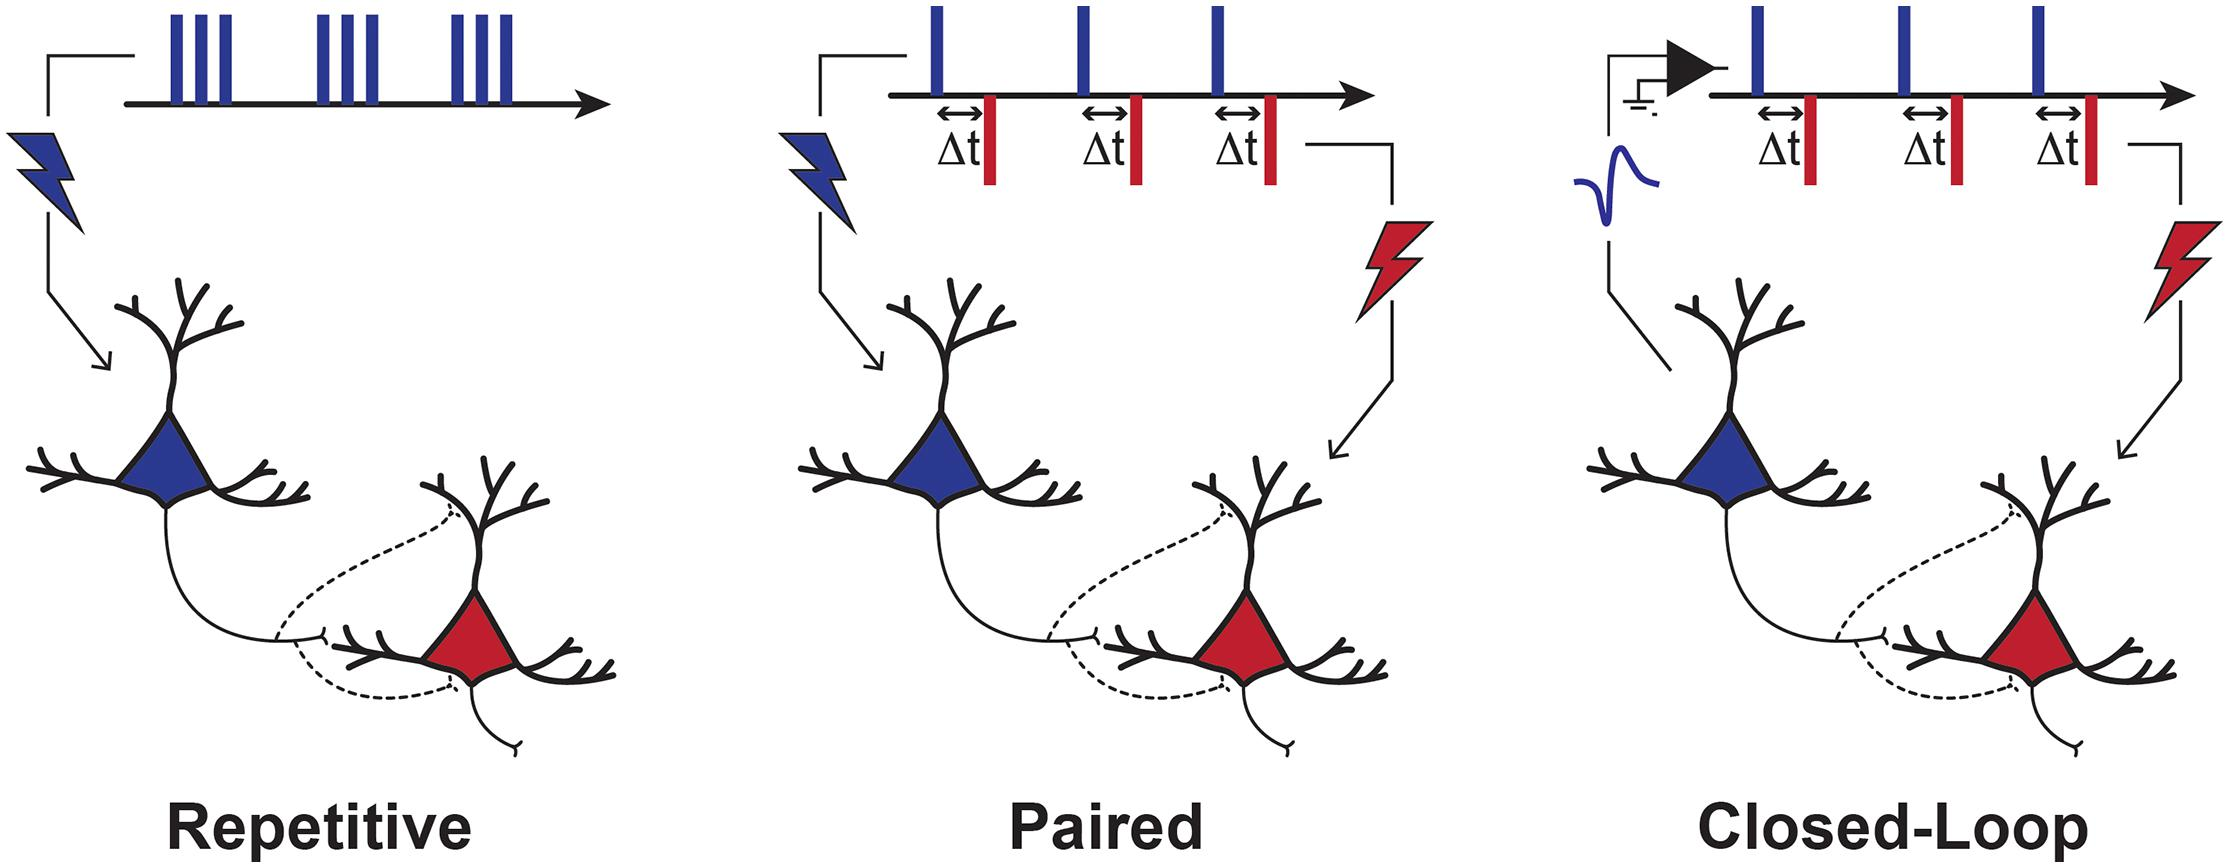
\includegraphics[width=0.9\linewidth]{Figure/Neuromodulation Paradigms.jpg}
    \end{center}
    \caption{\protect\cite{Ting2021} Stimulation paradigms to induce plasticity. Depiction of three main stimulation strategies used to induce plasticity.}
    \label{fig:Neuromodulation Paradigms}
\end{figure}

\subsubsection{Repetitive Stimulation}

Repetitive Stimulation (Figure \ref{fig:Neuromodulation Paradigms} left) involves repeatedly applying stimuli to the brain, especially to the primary motor cortex, to create lasting changes in synaptic strength and plasticity. It's often applied using non-invasive methods such as transcranial direct current stimulation (tDCS) and transcranial magnetic stimulation (TMS), with protocols like repetitive TMS (rTMS) and theta burst stimulation (TBS).

These methods tweak cortical excitability and restore a balanced interhemispheric inhibition. However, they have limitations in terms of spatial precision, and changes in cortical excitability may not always lead to long-term functional improvements. This can compromise their overall effectiveness, especially in cohorts with inter-individual variability \cite{Ting2021}.

\subsubsection{Paired Stimulation} 

Paired Stimulation (Figure \ref{fig:Neuromodulation Paradigms} center), as seen in methods like Paired Associative Stimulation (PAS) \cite{Alder2019}, synchronizes perisynaptic neuronal activity using a combination of TMS over the motor cortex and non-invasive electrical stimulation of the spinal cord or peripheral nerves. 

This method aims to modulate cortical excitability and induce spike-timing-dependent plasticity. However, the effectiveness of paired stimulation varies among subjects, requiring a deeper understanding of the brain's state to achieve precise temporal coordination during stimulation and induce plasticity \cite{Ting2021}.

\subsubsection{Closed Loop Stimulation}

Given the intricate and diverse organization of the nervous system, employing more precise stimulation techniques may prove more effective in inducing plasticity and, concurrently, lead to neural reorganization with greater functional benefits.

Closed loop stimulation paradigm (Figure \ref{fig:Neuromodulation Paradigms} right) represents a promising avenue in this regard, where the delivery of neural stimulation is dynamically adjusted based on real-time monitoring of ongoing brain activity. 
Unlike open loop approaches, closed loop stimulation systems can detect specific neuronal events or brain states and tailor the timing and intensity of stimulation accordingly. This refinement, for example in the  Deep Brain Stimulation (DBS), contributes to enhanced precision, efficacy, and overall functional benefits.
Both Behavior-Controlled stimulation and EEG-Controlled stimulation infer voluntary effort, but the latter doesn’t depend on physical movement. However, while offering advantages through adaptability and precision in enhancing natural patterns of neuronal and muscular activity in stroke patients, limitations in effectiveness persist for non-moving or atypical patients.
Closed loop stimulation can be employed in therapeutic neuroprostheses and Brain-Computer Interfaces (BCI), also using invasive methods. Studies have shown that spike-triggered intracortical stimulation is effective in improving functional recovery, reactivating paralyzed muscles, and inducing plasticity \cite{Ting2021}.

Nevertheless, despite recent results demonstrated the capabilities of a personalized closed loop approach (called Activity Dependent Stimulation, ADS), to better entrain network activity compared to standard open loop random stimulation \cite{Guggenmos2013,Averna2020,Averna2021}, the deployment of closed loop systems, whether invasive or non-invasive, is hindered by technical complexities and restricted accessibility.
 
\subsection{Neuroprostheses}

Neuroprosthetics represent a cutting-edge field at the intersection of neuroscience, engineering, and medical technology concerned with developing prosthetic devices that interact with the nervous system. 
These bioelectronic devices can also be classified as bio-hybrid systems, considering the human factor as a biological component, and they can be implemented using both open loop and closed loop approaches.

These neuroprostheses aim to substitute or regulate portions of the nervous system where electrophysiological activity has been disrupted due to neurodegenerative and neuropsychiatric disorders, after stroke, Traumatic Brain Injury (TBI), or Spinal Cord Injury (SCI).
They are currently employed to treat motor and sensory disorders, but lately, cognitive deficits have also become a target \cite{Gupta2023}.

Recent advancements have led to the development of closed loop neuromorphic neuroprostheses \cite{Famm2013,Reardon2014}, capable of establishing bidirectional communication between the artificial and biological components \cite{Broccard2017} and delivering output through electrical, chemical, or optogenetic stimulation \cite{Christensen2022}.

Indeed, a closed loop architecture is essential for developing a neuroprosthesis \cite{Levi2018,Buccelli2019}, specifically a type known as brain-prostheses. These brain-prostheses are designed to replicate the electrical activity of biological neural networks, facilitating interaction between the artificial and biological components \cite{Bonifazi2013}. They also enable the replacement of a damaged brain area with an artificial device capable of providing an interpretable response to the nervous system after processing the acquired neural signals.

\begin{figure}[ht!]
    \begin{center}
    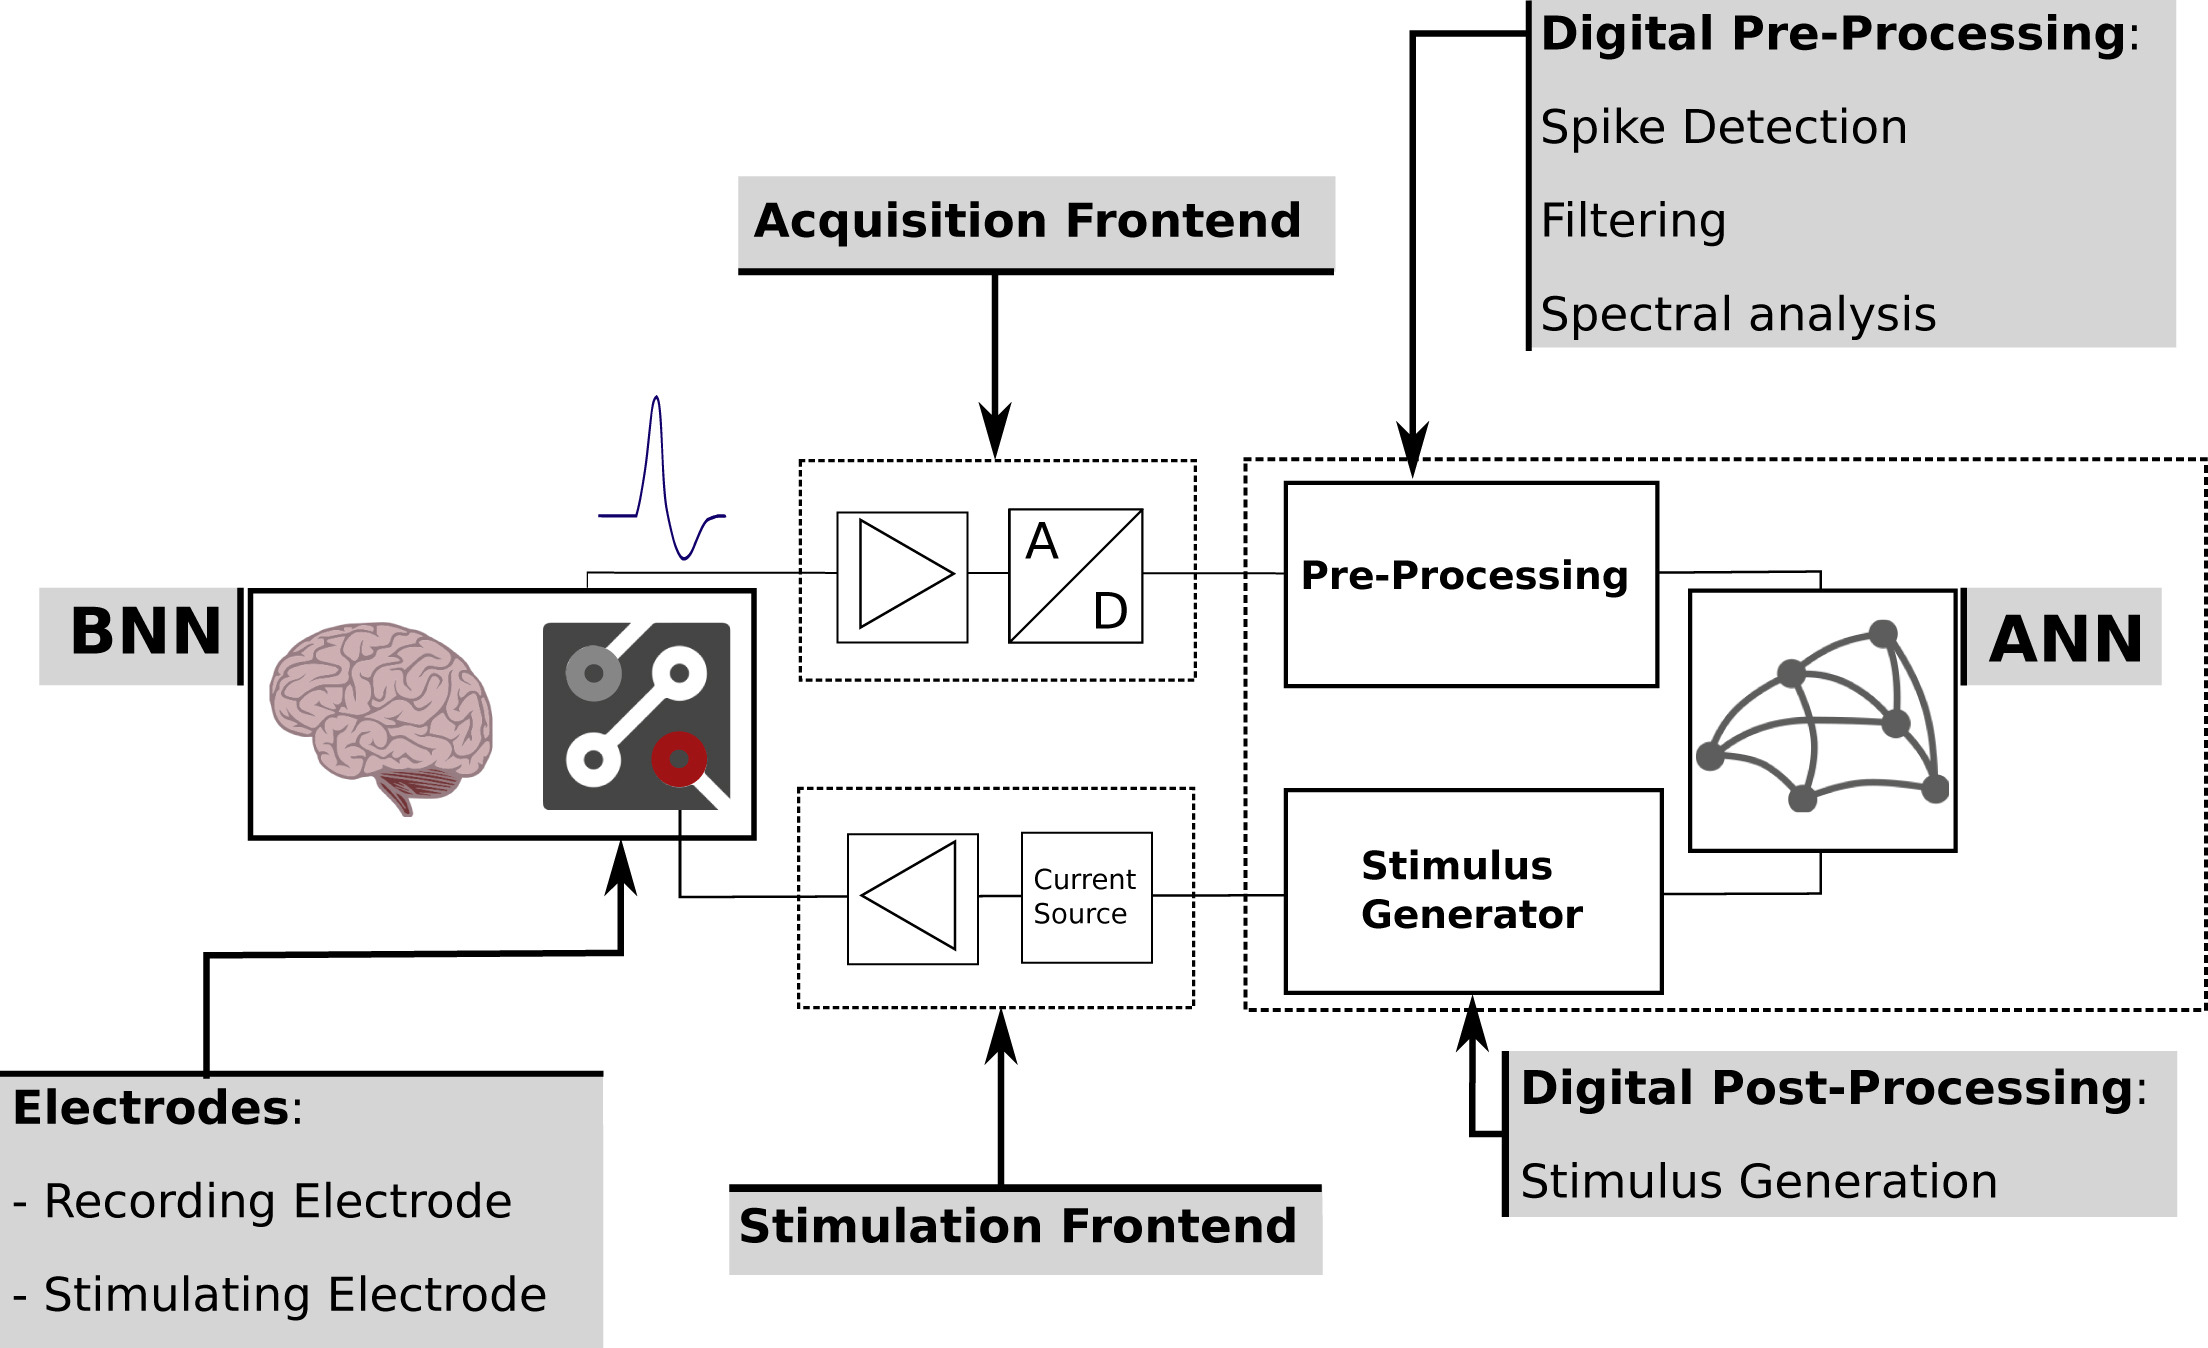
\includegraphics[width=0.9\linewidth]{Figure/Bio-Hybrid Closed Loop System.jpg}
    \end{center}
    \caption{\protect\cite{George2020} Setup of a bio-hybrid closed loop system. The Biological Neural Network (BNN) and the Artificial Neural Network (ANN) are connected through stimulation and recording electrodes. The BNN activity is amplified and digitized before extracting informative features, which are then fed as input into the ANN. Then, the ANN activity defines the stimulation protocol to be applied to the BNN through the stimulation electrodes. This mutual influence creates a bidirectional communication.}
    \label{fig:Bio-Hybrid Closed Loop System}
\end{figure}

As depicted in Figure \ref{fig:Bio-Hybrid Closed Loop System}, the neuromorphic artificial component of the bio-hybrid system can consist of an Artificial Neural Network (ANN) that simulates the architecture and complex dynamics of biological neurons.\\
These ANNs can be of two types: bio-inspired or bio-mimetic. The former category includes computational systems inspired by biological architectures that use simplified neuron models, for example, to execute accelerated time simulations in the field of artificial intelligence \cite{Tavanaei2019}. The latter category includes realistic models that imitate biological neurons and faithfully reproduce their features using complex neuron models operating at biological timescales. These models are employed to simulate neural network dynamics and/or conduct bio-hybrid experiments.

In the family of ANNs, Spiking Neural Networks (SNNs) are the most biophysically plausible, as they can reproduce neuronal phenomena, ranging from electrophysiological activity in single cells (soma, axon, and dendrites) to the plasticity of the network. By integrating bio-mimetic with multi-compartment models, it becomes possible to model also the morphological characteristics of a neuron and design an SNN capable of reproducing the spatial configuration of neurons and associated spike timing and morphology.

Recently, a biomimet\-ic Spiking Neural Network (SNN) has been utilized to develop an electroceutical solution \cite{DiFlorio2023} that, in contrast to \cite{Buccelli2019}, employed Hodgkin-Huxley neurons. The SNN, consisting of 1024 unconnected neurons, dictated the pace for open-loop stimulation to the brains of rats as part of a post-stroke rehabilitation protocol.

Most of the current solutions for biomimetic SNN simulations are soft\-ware-based, such as NEURON, NEST, and Brian2 \cite{HinesCarnevale2001,GewaltigDiesmann2007,Stimberg2019}, and they are not suited for real-time emulation and interaction at the biological timescale due to the high computational time required.

On the contrary, hardware-based SNNs, such as TrueNorth, BrainScaleS-2, SpiNNaker, and Loihi \cite{Merolla2014,Pehle2022,Painkras2013,Davies2018,Stradmann2022}, are able to perform real-time emulation and can be either analog, hence less power-hungry, or digital, hence more flexible and more suited for prototyping.

This work focuses on tuning the parameters of a new real-time hardware-based SNN, Bi{\oe}muS \cite{Beaubois2023}, to be used for delivering novel personalized electrical stimulations in pre-clinical studies.

\section{Biological Modeling}

Models are frequently employed across various disciplines to explore intricate problems, offering a means to circumvent constraints and external influences. Specifically, biological models of the human body serve as experimental systems designed to replicate specific biological processes both physiological and pathological. These models generally fall into two categories: in-vitro (cell-based) and in-vivo (animal-based).

\subsection{In-vitro 2D models}

In-vitro two-dimensional (2D) cultures are cellular models cultivated on flat surfaces, such as culture dishes or multi-well plates, allowing for consistent control of the environment outside of a living organism. The advantage of this method lies in the simplicity of its handling and experimental measurement processes, providing a wide range of established cell lines. Furthermore, it offers simplified and highly reproducible systems to investigate cellular and molecular interactions. However, this model is often limited in terms of physiological coherence, as it does not fully reproduce the complexity of tissues and organs.

\subsection{In-vitro 3D models}

In-vitro three-dimensional (3D) cultures are cellular models cultivated in a device that allows cells to organize and interact in three dimensions, thereby replicating tissues and organs in a more coherent manner \cite{Pampaloni2007,BreslinO’Driscoll2013,Duval2017}. 

For example, in-vitro 3D cultures are widely used to study the human brain, such as through organoid cultures that can reproduce structures of certain brain areas \cite{Kim2020}.

A more complete model involves the design of Organ-On-Chip (OOC) systems, which are microfluidic platforms incorporating cells and tissues in a three-dimensional arrangement to replicate, in vitro, the complex architecture and interactions present in real human organs \cite{Huh2011,Ma2021}.

\subsection{In-vivo models}

In-vivo models for human biology modeling often involve animals, such as rodents \cite{Peters2007} and non-human primates. To date, they are of fundamental importance for future applications in humans. These experiments explore various biological processes, diseases, and drug responses within the authentic physiological context of living organisms, exhibiting fewer limitations compared to in-vitro cultures.

While in-vivo experiments account for the complex interactions in a living organism, thus providing a more coherent approach, they are often significantly more complex to conduct compared to in-vitro 2D experiments. Notably, in-vivo studies demand rigorous adherence to ethical protocols to ensure both animal welfare and the scientific integrity of the research conducted.

\subsubsection{In-vivo models of Stroke}

Various rodent models are employed for testing neuroprotective therapies and exploring reparative mechanisms in the brain post-stroke. These models aim to create reproducible infarcts with minimal surgical intervention to decipher cell death mechanisms and assess neuroprotective strategies. Ischemic stroke animal models are broadly categorized as global, focal, and multifocal \cite{Graham2004}:
\begin{itemize}
    \item In cases of global ischemia, there is a reduction in blood flow across the entire brain. It can be complete, involving the total cessation of global blood flow for a period, or incomplete, entailing a significant reduction in blood flow to impede normal metabolism and function;
    \item Focal strokes target specific brain regions and are prominently represented by middle cerebral artery occlusion (MCAO), where a blood clot is introduced through the internal carotid to occlude the MCA, temporarily or permanently reducing blood flow to a specific hemisphere. This model closely mimics human ischemic stroke \cite{Garcia1993,Tsuji2013,Zhang2013}. Other methods, such as the stereotaxic injection of the vasoconstrictive peptide endothelin-1 (ET-1) into the cortex, precisely localize effects to specific brain regions, supporting functional recovery \cite{Frost2006,Fang2010};
    \item Multifocal ischemic strokes induce reduced cerebral blood flow in multiple areas using various methods such as embolization, microspheres, or photochemically induced thrombi \cite{McAuley1995,Traystman2003}.
\end{itemize}

In this work, a rodent model of focal ischemic stroke induced by ET-1 was employed. This method is known for being less invasive, having low mortality, and inducing direct focal ischemia in both deep and superficial brain regions \cite{Sharkey1993}. The lesion was performed in the caudal forelimb area (CFA), a region within the cortical sensorimotor system. 

This area in the frontal cortex shares many characteristics with the primary motor cortex (M1) of primates, and injuries to M1 are known to lead to long-term impairments in reaching and grasping functions \cite{Nishibe2010}. Traditionally, it was believed that such impairments occurred because M1 provides substantial outputs to the motor apparatus in the spinal cord, directly affecting motor output function. However, M1 also has significant interconnections with the primary somatosensory cortex (S1) located in the parietal lobe (Figure \ref{fig:Brain-Machine-Brain Interface}A). Long-range corticocortical fibers from S1 play a crucial role in providing information to M1 regarding the limb's position in space. Consequently, impaired motor performance resulting from an injury to M1 could be also attributed, at least partially, to a disruption in communication between the somatosensory and motor cortex \cite{Friel2005}.

\begin{figure}[ht!]
    \begin{center}
    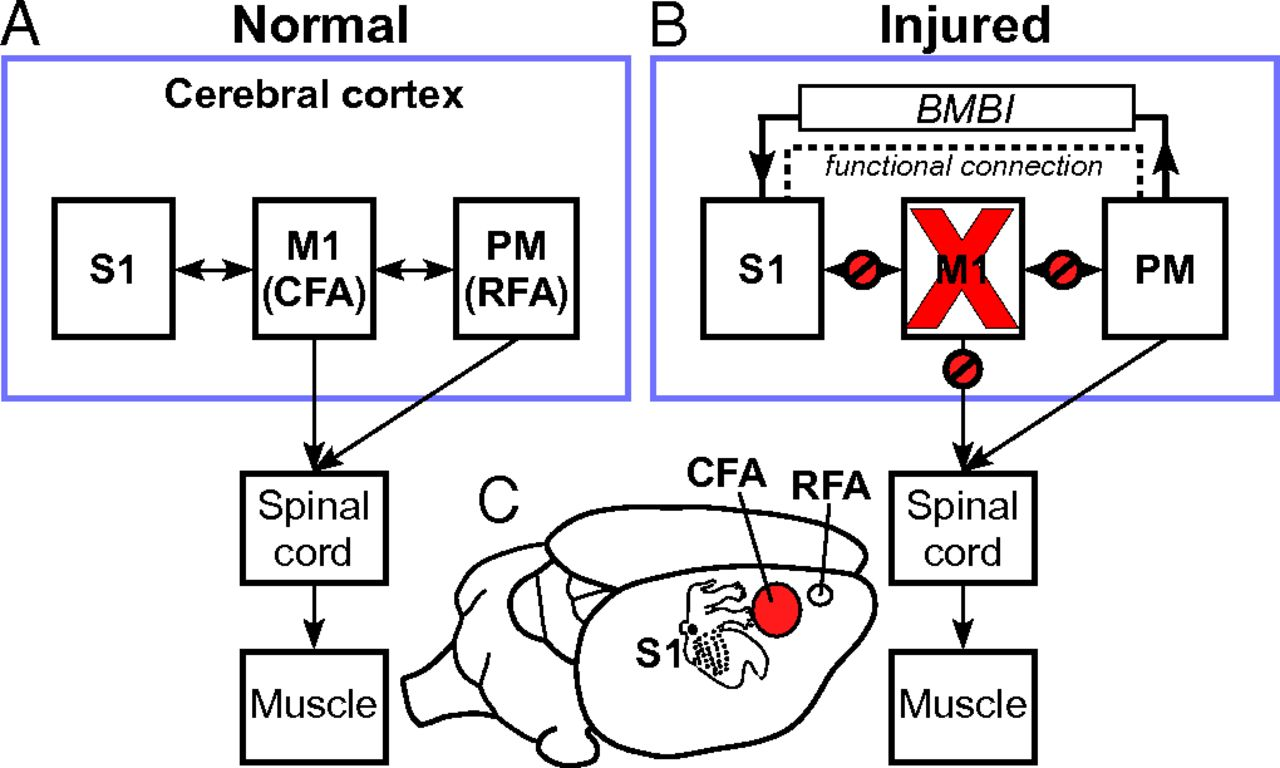
\includegraphics[width=0.9\linewidth]{Figure/Brain-Machine-Brain Interface.jpeg}
    \end{center}
    \caption{\protect\cite{Guggenmos2013} Theoretical model of neuroprosthetic treatment approach after brain injury. (A) Normal connectivity of M1, S1, and PM. Both M1 (CFA in rat) and PM (RFA in rat) send substantial outputs to the spinal cord via the corticospinal tract. Also, extensive reciprocal connections exist between M1 and PM, as well as between M1 and S1. (B) Effects of focal M1 injury on brain connectivity and the hypothetical effect of a BMBI to restore somatosensory-motor communication. An injury to M1 disrupts the corticocortical communication between M1 and S1 (and between M1 and PM). Thus, the uninjured PM, which contains corticospinal neurons as well, might be exploited. The dotted line indicates enhanced functional connection between PM and S1 established after treatment with a BMBI.(C) Location of target areas in rat cerebral cortex. A topographic map of the somatosensory representation in S1 is superimposed on the cortex.}
    \label{fig:Brain-Machine-Brain Interface}
\end{figure}

In particular, the rostral forelimb area (RFA) is believed to contribute to the recovery of function after an injury to M1 \cite{Nishibe2010,Conner2005,Rouiller1993}, and it was indeed exploited in \cite{Guggenmos2013} for the development of a closed-loop brain–machine–brain interface (BMBI)(Figure \ref{fig:Brain-Machine-Brain Interface} B,C). The RFA is a premotor region in the rodent's frontal cortex that shares many characteristics with the premotor (PM) cortex of primates. Although PM areas also have long-range corticocortical connections with somatosensory areas, in intact animals, these connections appear to be relatively weak compared to M1's connections with the somatosensory cortex \cite{Rouiller1993,Dancause2005,Fang2005}.

\section{Artificial Modeling}

Artificial models, inspired by nature, play a crucial role in simplifying and simulating specific aspects of systems, addressing technological challenges across various fields. Bio-inspired Artificial Neural Networks (ANNs), emulating the architecture of the human brain, excel in diverse signal processing tasks. Image recognition, classification, natural language processing, speech recognition, and time-series prediction tasks often leverage Feedforward Neural Network (FNN) \cite{Svozil1997}, Convolutional Neural Network (CNN) \cite{O'SheaNash2015}, or Recurrent Neural Network (RNN) \cite{MedskerJain1999} for information processing. Additionally, SNNs, introduced in the section "Neuroprosthesis", represent a more biologically accurate form of ANNs, simulating the behavior of biological neurons and their interactions through action potentials or spikes \cite{Ghosh-DastidarAdeli2009}.

\subsection{Neuron models}

Differently from the mere bio-inspired neurons used in artificial intelligence (for FNN, CNN and RNN), bio-mimetic neurons aim to faithfully reproduce phenomena happening in nature.

The model proposed by \cite{HodgkinHuxley1990}, known as the HH model, is considered the first biologically meaningful mathematical neuron model. Derived from experiments conducted on the squid giant axon, this model incorporates three currents: sodium, potassium, and leak current. The experiments revealed that the ionic permeability of the membrane is highly dependent on the membrane potential. As a result, the HH model was developed based on the voltage-dependent properties of the membrane to simulate the generation of an action potential. The opening and closing of ion channels are represented as variable conductance determined by the voltage.

Figure \ref{fig:HH model Electric Circuit} depicts the schematic of the Hodgkin-Huxley model whose behaviour is described by the Equation \ref{eq:HH model}.

\begin{figure}[ht!]
    \begin{center}
    \begin{circuitikz}
    \draw (3,-3) node[circle, fill=black, draw, inner sep=1pt]{};
    \draw (3,-3) node[below] {Intracellular};
    \draw (3,-3) -- (3,-2);
    \draw (3,3) node[circle, fill=black, draw, inner sep=1pt]{};
    \draw (3,3) node[above] {Extracellular};
    \draw (3,3) -- (3,2);
    \draw (0,-2) -- (6,-2);
    \draw (0,2) -- (6,2);
    
    % Capacitor
    \draw (6,2) to[C, l=$C_m$] (6,-2);

    % Sodium branch
    \draw (0,0) to[vR, l=$g_{Na}$] (0,2);
    \draw (0,-2) to[battery1] (0,0);
    \draw (-0.90,-1.3) node[circle, label=$E_{Na}$, inner sep=1pt]{};
    
    % Potassium branch
    \draw (2,0) to[vR, l=$g_{K}$] (2,2);
    \draw (2,-2) to[battery1, invert] (2,0);
    \draw (1.10,-1.3) node[circle, label=$E_{K}$, inner sep=1pt]{};

    % Leak branch
    \draw (4,0) to[R, l=$g_{Leak}$] (4,2);
    \draw (4,-2) to[battery1, invert] (4,0);
    \draw (3.10,-1.3) node[circle, label=$E_{Leak}$, inner sep=1pt]{};

    \draw [>=stealth, <->] (8,-3) -- (8,3);
    \draw (8.4,-0.3) node[above] {$V_{m}$};

    \end{circuitikz}
    \end{center}
    \caption{Electrical equivalent circuit of HH model representing $Na^{+}$, $K^{+}$ ionic currents and leakage current as a basic neuron model. $V_{m}$ is the membrane potential, $C_{m}$ is the membrane capacitance, $g_{Na}$ and $g_{K}$ the conductance of voltage-dependent ion channels, $E_{Na}$, $E_{K}$ and $E_{Leak}$ are the reversal potentials and $g_{Leak}$ a voltage independent conductance.}
    \label{fig:HH model Electric Circuit}
\end{figure}

\begin{equation}
C_m \frac{dV_m}{dt}=-(I_{Na}+I_{K}+I_{Leak})
\label{eq:HH model}
\end{equation}

where $I_{Na}$ is the sodium current, $I_{K}$ the potassium current, $I_{Leak}$ the leakage current.

Due to the complexity of the HH model, which relies on high-dimensional nonlinear differential equations, simpler models have been developed. These simplified models replicate neural dynamics using reduced equations, often incorporating threshold and reset mechanisms to generate action potentials.

Both FitzHugh-Nagumo [FitzHugh, 1955, FitzHugh, 1961, Nagumo et al., 1962] and Morris-Lecar [Morris and Lecar, 1981] models reduce the number of variables and equations compared to the HH model, capturing essential features of excitable cells while sacrificing some biophysical accuracy. These simplifications make FitzHugh-Nagumo and Morris-Lecar models suitable for certain applications where computational efficiency is crucial and detailed biophysical accuracy is not essential. 

Even further simplification of neuronal dynamics is found in the family of Integrate-and-Fire (IF) models  \cite{Abbott1999}. In the IF model, a spike is generated each time the membrane potential crosses the threshold, and it is reset to the resting potential only after this event. The family includes variations like Leaky Integrate-and-Fire (LIF) \cite{GerstnerKistler2002}, Exponential Integrate-and-Fire (EIF) \cite{Fourcaud-Trocmé2003}, and Adaptive Exponential Integrate-and-Fire (AdEx) \cite{GerstnerBrette2009} models that introduce specific modifications to enhance biological plausibility while maintaining computational efficiency.

A model with significantly better biological plausibility is the Izhikevich (IZ) model \cite{Izhikevich2003}, capable of reproducing various neuron families (as illustrated in Figure \ref{fig:Izhikevich Spiking Neuron Families}), while remaining computationally convenient.

\begin{figure}[ht!]
    \begin{center}
    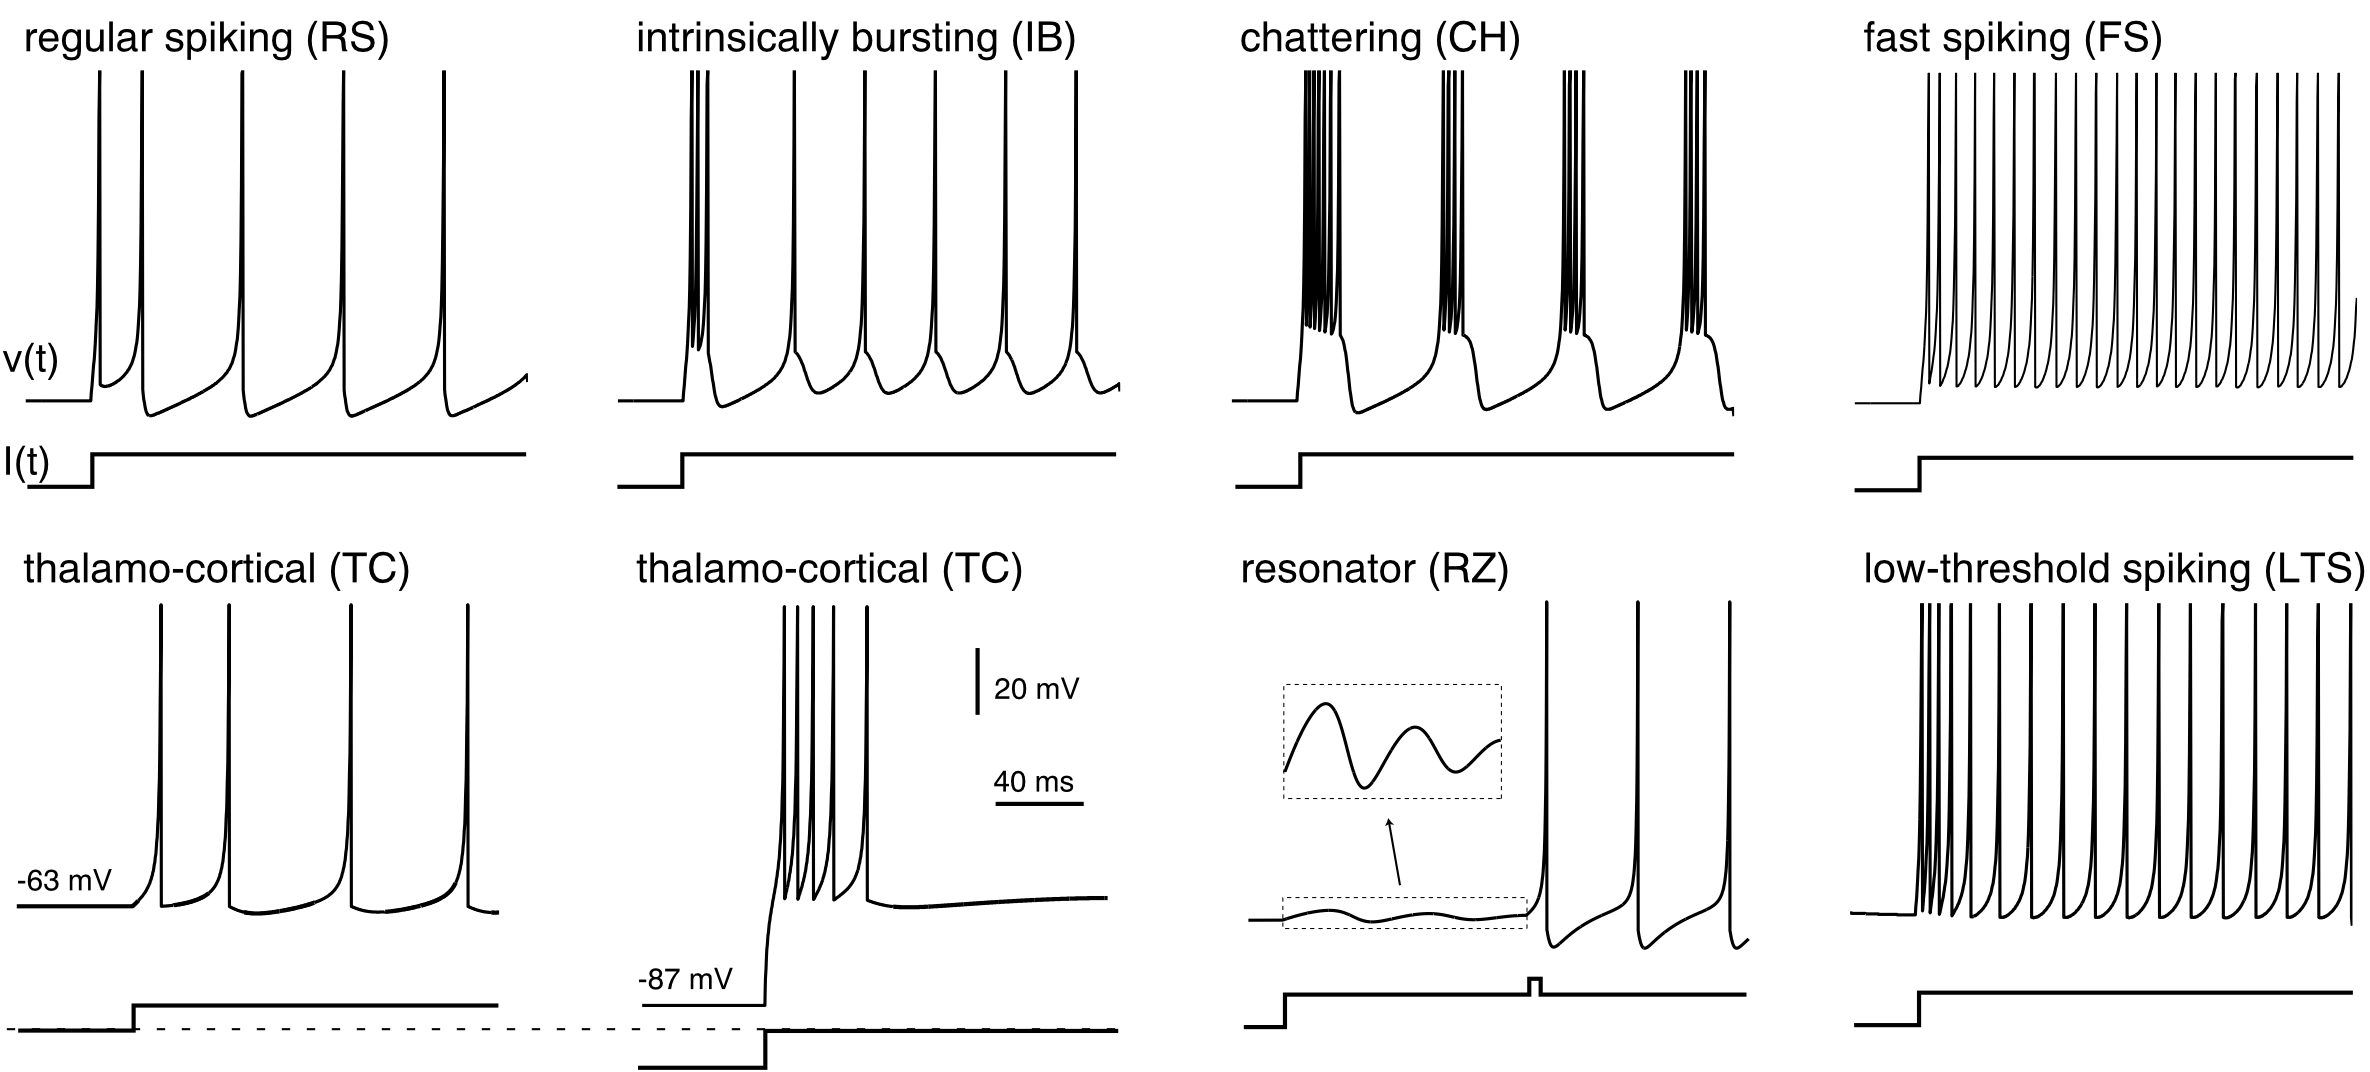
\includegraphics[width=0.9\linewidth]{Figure/Izhikevich Spiking Neuron Families.jpg}
    \end{center}
    \caption{\protect\cite{Izhikevich2003} Spiking neuron families obtained using different values of the parameters in the Izhikevich model.}
    \label{fig:Izhikevich Spiking Neuron Families}
\end{figure}

However, while biophysical meaningfulness is a critical requirement for true bio-mimetic modeling, the implementation on a numeric platform introduces a dilemma between biological coherence and practicality. Despite the IZ model presenting an appealing compromise between implementation cost and biological coherence, it lacks biological meaningfulness and deviates from bio-realism, impacting its ability to predict the behavior of neurons in specific conditions \cite{Brette2015}.

In this work, the highest biological coherence and meaningfulness were achieved by utilizing a SNN with conductance-based HH neurons, representing the best bio-mimetic model.

\subsubsection{Single-compartment models}

The single-compartment model of a neuron is commonly employed in computational neuroscience, approximating the neuron to a point in space and neglecting the spatial dimension. It is represented as a large membrane capacitance in parallel with a series of conductances and batteries, as illustrated in Figure \ref{fig:HH model Electric Circuit}. The temporal dynamics of the membrane potential, capturing the essential mechanisms of $Na^{+}$ and $K^{+}$ channels, can be described using the HH model by Equation \ref{eq:HH model}.

More specifically, each ionic current can be represented by Equation \ref{eq:General Ion Current}:

\begin{equation}
I_{ion} = g_{ion} m^{{p}_{ion}}_{ion} h^{{q}_{ion}}_{ion} (V-E_{ion})
\label{eq:General Ion Current}
\end{equation}

where $I_{ion}$ is the ionic current, $g_{ion}$ is the maximum conductance of the ion channel, $m^{{p}_{ion}}$ and $h^{{q}_{ion}}$ are respectively the activation and inactivation variables, each taking a probability value between 0 and 1, $v$ is the membrane voltage and $E_{ion}$ is the equilibrium potential of the ion. 

In general, depending on the desired neuron model, several ion channels can be included. In the case represented in Figure \ref{fig:HH model Electric Circuit} and Equation \ref{eq:HH model}, three currents are considered, corresponding to Equations \ref{eq:Sodium Ion Current}, \ref{eq:Potassium Ion Current}, \ref{eq:Leakage Current}:

\begin{equation}
I_{Na} = g_{Na} m^{3}_{Na} h_{Na} (V-E_{Na})
\label{eq:Sodium Ion Current}
\end{equation}

\begin{equation}
I_{K} = g_{K} m^{4}_{K} (V-E_{K})
\label{eq:Potassium Ion Current}
\end{equation}

\begin{equation}
I_{Leak} = g_{Leak} (V-E_{Leak})
\label{eq:Leakage Current}
\end{equation}

The values of the activation and inactivation variables of the voltage-gated ion channels are described by equations representing different sigmoids for each channel. The formulae are expressed using the following formalism (Equation \ref{eq:General Gating Particle}):

\begin{equation}
\frac{dp_{i}}{dt} = \alpha_{i}(V)(1-p_{i})-\beta_{i}(V)p_{i}
\label{eq:General Gating Particle}
\end{equation}

where $\alpha$ and $\beta$ are voltege-dependent parameters. Introducing the steady-state solution: 

\begin{equation}
p_{i, t\to\infty}(V) = \frac{\alpha_{i}(V)}{\alpha_{i}(V)+\beta_{i}(V)}
\label{eq:Steady-state Solution Gating Particle}
\end{equation}

and the time constant formulae:

\begin{equation}
\tau_{i}(V) = \frac{1}{\alpha_{i}(V)+\beta_{i}(V)}
\label{eq:Time Constant Gating Particle}
\end{equation}

the Equation \ref{eq:General Gating Particle} can be written as follow:

\begin{equation}
\frac{dp_{i}}{dt} = \frac{p_{i, \infty}(V)-p_{i}}{\tau_{i}(V)}
\label{eq:Alternative General Gating Particle}
\end{equation}

\subsubsection{Multi-compartmental models}

The multi-compartmental model provides a more biologically realistic approach, enabling the analysis of complex spatial details and behaviors of neurons. In particular, it allows the investigation of biophysical phenomena and neurodegenerative diseases that affect specific regions of the neurons. 

Thus, the neuron is discretized into more or fewer compartments, depending on the desired level of fidelity or abstraction, following the cable theory. Each segment is then described by an electrical equivalent circuit, such as the HH model, linked to each other by resistors simulating axoplasmic resistance (as depicted in Figure \ref{fig:Multi-compartimental Model}).

\begin{figure}[ht!]
    \begin{center}
    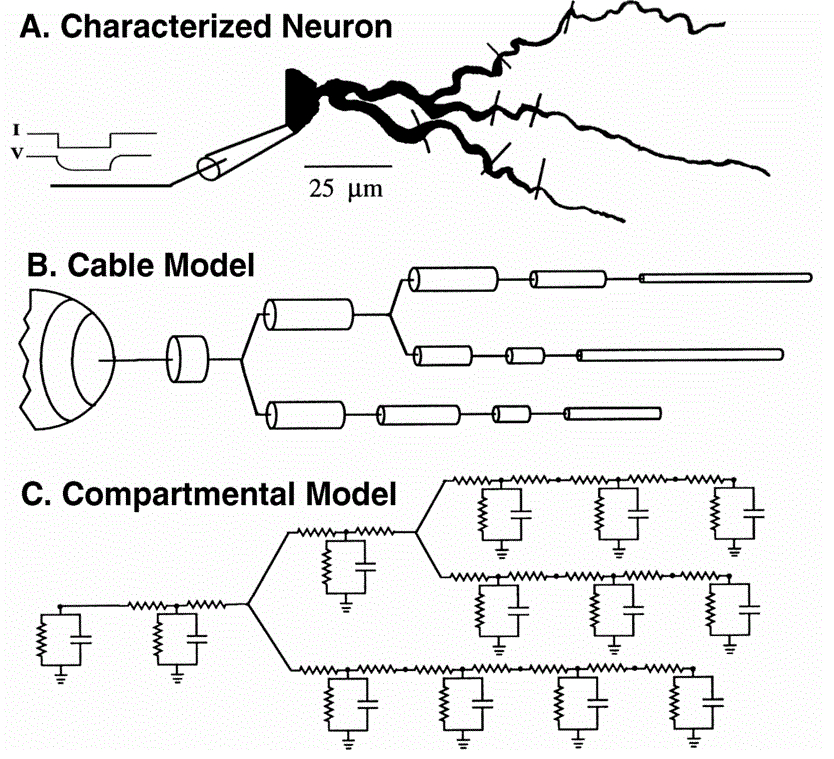
\includegraphics[width=0.9\linewidth]{Figure/Multi-compartimental Model.jpg}
    \end{center}
    \caption{Electrical equivalent circuit of multicompartmental neuron model. The neuron (A) is first discretized into cylindrical compartments of various lengths and radii (B), and then each segment is represented by its own equivalent electrical circuit (C). Extracted from [Christof Koch, Idan Segev, CC BY-SA 3.0 (https://creativecommons.org/licenses/by-sa/3.0), via Wikimedia Commons]}
    \label{fig:Multi-compartimental Model}
\end{figure}

Given that each element of the neuron corresponds to a different compartment, it's possible to describe the properties of each segment with a specific HH model. This crucial feature makes the multi-compartmental models even more biologically meaningful compared to the single-compartment models.

\subsection{Noise models}

A peculiar behaviour of the neurons is their capacity to generate spontaneous stimulus-independent spikes. Thus, is fundamental to reproduce this property in an artificial model. 

Commonly, this behavior is modeled by injecting a noisy current based on a normal distribution into the neuron, eliciting more or fewer spikes depending on its amplitude and standard deviation. However, it's possible to generate a current more similar to the synaptic noise observed in biology by fluctuating the conductances of ion channels \cite{Destexhe2001,Tuckwell2002}. Equation \ref{eq:Biomimetic Noise} expresses this biomimetic noise, which is based on the Ornstein-Uhlenbeck process.

\begin{equation}
\frac{di_{noise}(t)}{dt} = \theta(\mu-i_{noise}(t)) + \sigma\frac{dW(t)}{dt}
\label{eq:Biomimetic Noise}
\end{equation}

where $i_{noise}$ is the noisy current, $\theta$ and $\sigma$ define respectively the amplitude and deviation of the noise, $\mu$ is a constant adding drift, and $\frac{dW(t)}{dt}$ denotes the Wiener process.

\subsection{Synapse models}

Achieving a biophysically realistic model of the spike implies modeling the synapses as well. Among all the synapse models present in the literature, the one proposed by \cite{Destexhe1998} is the most biomimetic and biologically meaningful. Four types of synaptic receptors responsible for fast and slow excitation (AMPAR and NMDAR) and fast and slow inhibition (GABA\textsubscript{A}R and GABA\textsubscript{B}R) are modeled. It is a conductance-based model, and the synaptic currents generated by the receptors are expressed through Equations \ref{eq:AMPAR Synaptic Current}, \ref{eq:NMDAR Synaptic Current}, \ref{eq:GABAAR Synaptic Current} and \ref{eq:GABABR Synaptic Current}, and visualized in Figure \ref{fig:Destexhe Synaptic Models}.

\begin{equation}
I_{AMPA} = g_{AMPA} r (V-E_{AMPA})
\label{eq:AMPAR Synaptic Current}
\end{equation}

\begin{equation}
I_{NMDA} = g_{NMDA} r B(v) (V-E_{NMDA})
\label{eq:NMDAR Synaptic Current}
\end{equation}

\begin{equation}
I_{GABA_{A}} = g_{GABA_{A}} r (V-E_{GABA_{A}})
\label{eq:GABAAR Synaptic Current}
\end{equation}

\begin{equation}
I_{GABA_{B}} = g_{GABA_{B}} r \frac{s^{n}}{s^{n}+K_{d}}(V-E_{GABA_{B}})
\label{eq:GABABR Synaptic Current}
\end{equation}

where $g_{AMPA}$, $g_{NMDA}$, $g_{GABA_{A}}$, $g_{GABA_{B}}$ are the maximum conductances of the receptors, $E_{AMPA}$, $E_{NMDA}$, $E_{GABA_{A}}$, $E_{GABA_{B}}$ are the equilibrium potentials, and $r$ and $s$ are the state variables for activation and inactivation of the receptors.

\begin{figure}[ht!]
    \begin{center}
    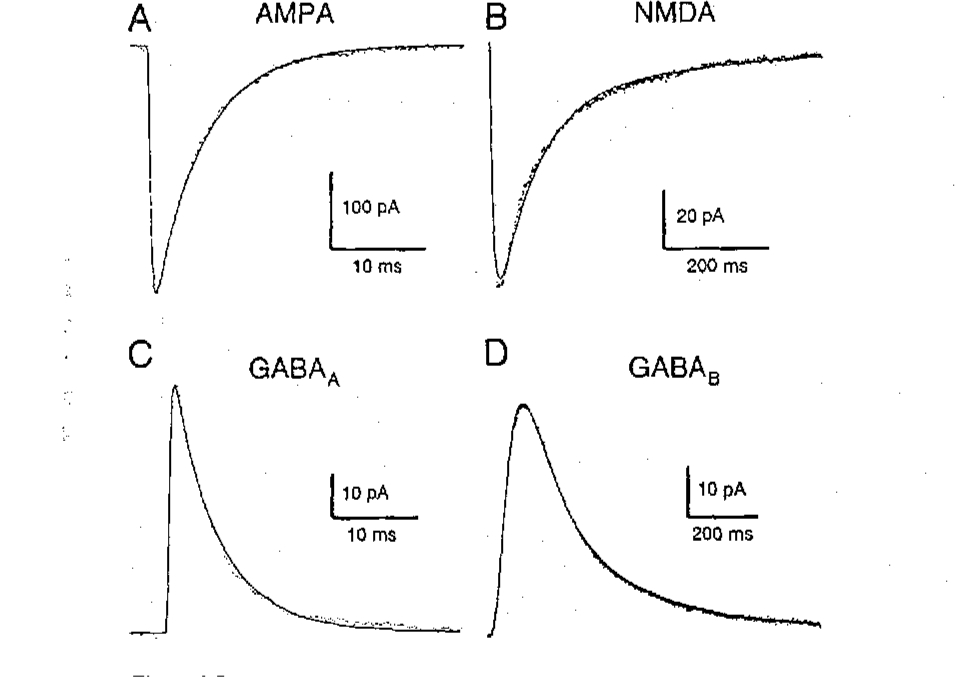
\includegraphics[width=0.9\linewidth]{Figure/Destexhe Synaptic Models.jpg}
    \end{center}
    \caption{\protect\cite{Destexhe1998} Post-synaptic currents. The curves represent the best fits of detailed kinetic models to averaged postsynaptic currents obtained from whole-cell recordings. (A) AMPAR current. (B) NMDAR current. (C) GABA\textsubscript{A}R current. (D) GABA\textsubscript{B}R current.}
    \label{fig:Destexhe Synaptic Models}
\end{figure}

For enhancing the biological fidelity and meaningfulness of the network, it's crucial to also mimic synaptic plasticity. Synaptic plasticity, in general, refers to the ability of synapses to change in strength over time and is linked to the learning capabilities of the network.

In neuroscience, Hebbian plasticity \cite{Hebb1949} is a fundamental principle that embodies the concept often expressed as "cells that fire together, wire together". This theory encompasses the most prevalent models of plasticity, including Short-Term Plasticity (STP), Spike-Timing-Dependent Plasticity (STDP), Long-Term Potentiation (LTP), and Long-Term Depression (LTD).

STP acts on short time scales (milliseconds to seconds), involving temporary increases or decreases in synaptic strength.

STDP operates over short to intermediate time scales, and the changes in synaptic strength are determined by the relative timing of spikes in pre- and postsynaptic neurons.

LTP and LTD mechanisms act on extended time scales. LTP results in a lasting reinforcement of synaptic connections induced by their repeated activation, contributing to memory formation. On the other hand, LTD leads to a weakening of synaptic connections when they are subjected to prolonged low-frequency stimulation or inactivity. This process plays a crucial role in homeostatic regulation, preventing excessive excitation caused by LTP.

\section{Summary}

This chapter introduces the main problems that the nervous system can face and the primary rehabilitation solutions to enhance stroke damage. It also covers the methods used to study the human nervous system, ranging from biological models to artificial ones. All this knowledge is essential for creating novel electroceutical treatments to deliver personalized stimulations.

The following chapters aim to delve into the steps performed in order to create a real-time hardware-based SNN that mimics the electrophysiological behavior of an in vivo Biological Neural Network (BNN). In particular, the next chapter will focus on characterizing the evoked activity, which will be used to study the effects of the lesion and traditional stimulation paradigms.
